\subsection{Der Mikrocontroller}
	Ein Mikrocontroller ist ein Ein-Chip-Computersystem, der einen Prozessor und Peripheriefunktionen beinhaltet. In den meisten Fällen befindet sich der Arbeits- und Programmspeicher teilweise oder auch komplett auf demselben Chip. 
	
	In der Industrie ist der Mikrocontroller bereits seit vielen Jahren ein nicht mehr wegzudenkendes Bauteil. Sie werden im Alltag in eingebetteten Systemen verwendet, zum Beispiel in Waschmaschinen, Fernsehgeräte und sogar im Fahrzeug als Steuergeräte für das Antiblockiersystem (ABS), Airbag usw.
	
	Mikrocontroller können in verschienden Sprachen programmiert werden. Welche sich jedoch am besten eignet, ist vom Anwendungsfall abhängig. Assembler eignet sich besonders, da es einen direkten Einstieg in die Hardware bietet und keine Abhängigkeiten zu anderen Compilern hat.\footnote{http://www.mikrocontroller.net/articles/AVR-Tutorial}. 
	
\subsection{Assembler}
	Ein Assembler ist ein Übersetzer für Programmcode, der sich aus Maschinenbefehlen zusammensetzt. In der Art der verwendeten Befehle besteht der wesentliche Unterschied zu allen anderen Programmiersprachen. 
	
	Während sich Befehle bei den Hochsprachen, wie beispielsweise Java und C++, in der Übersetzung aus mehreren Anweisungen im endgültigen Code zusammensetzen, wird der Assemblerbefehl durch den Assembler lediglich in die entsprechende Binärform übersetzt. Weiterhin ersetzt der Assembler Variablen durch die entsprechenden Speicheradressen\footnote{Vgl. http://assembler.hpfsc.de/}.
	
\subsection{MSC-8051}
	Der MSC-8051 ist die Bezeichnung einer von Intel vorgestellten Familie von 8-Bit-Mikrocontrollern.
	
	
	% \footnote{http://www.mikrocontroller.net/articles/8051}
	
	% \footnote{https://de.wikipedia.org/wiki/Intel_MCS-51}

\subsection{MCU 8051 IDE}
	Die MCU 8051 IDE ist eine grafische Entwicklungsumgebung für Mikrocontroller, die auf dem MSC-8051 basieren. Das folgende Bild stammt von der Homepage\footnote{http://www.moravia-microsystems.com/mcu-8051-ide/} der Entwicklungsumgebung. Es zeigt im Hintergrund den Aufbau der IDE und im Vordergrund einige Simulationsfeatures. 

	\begin{center}
		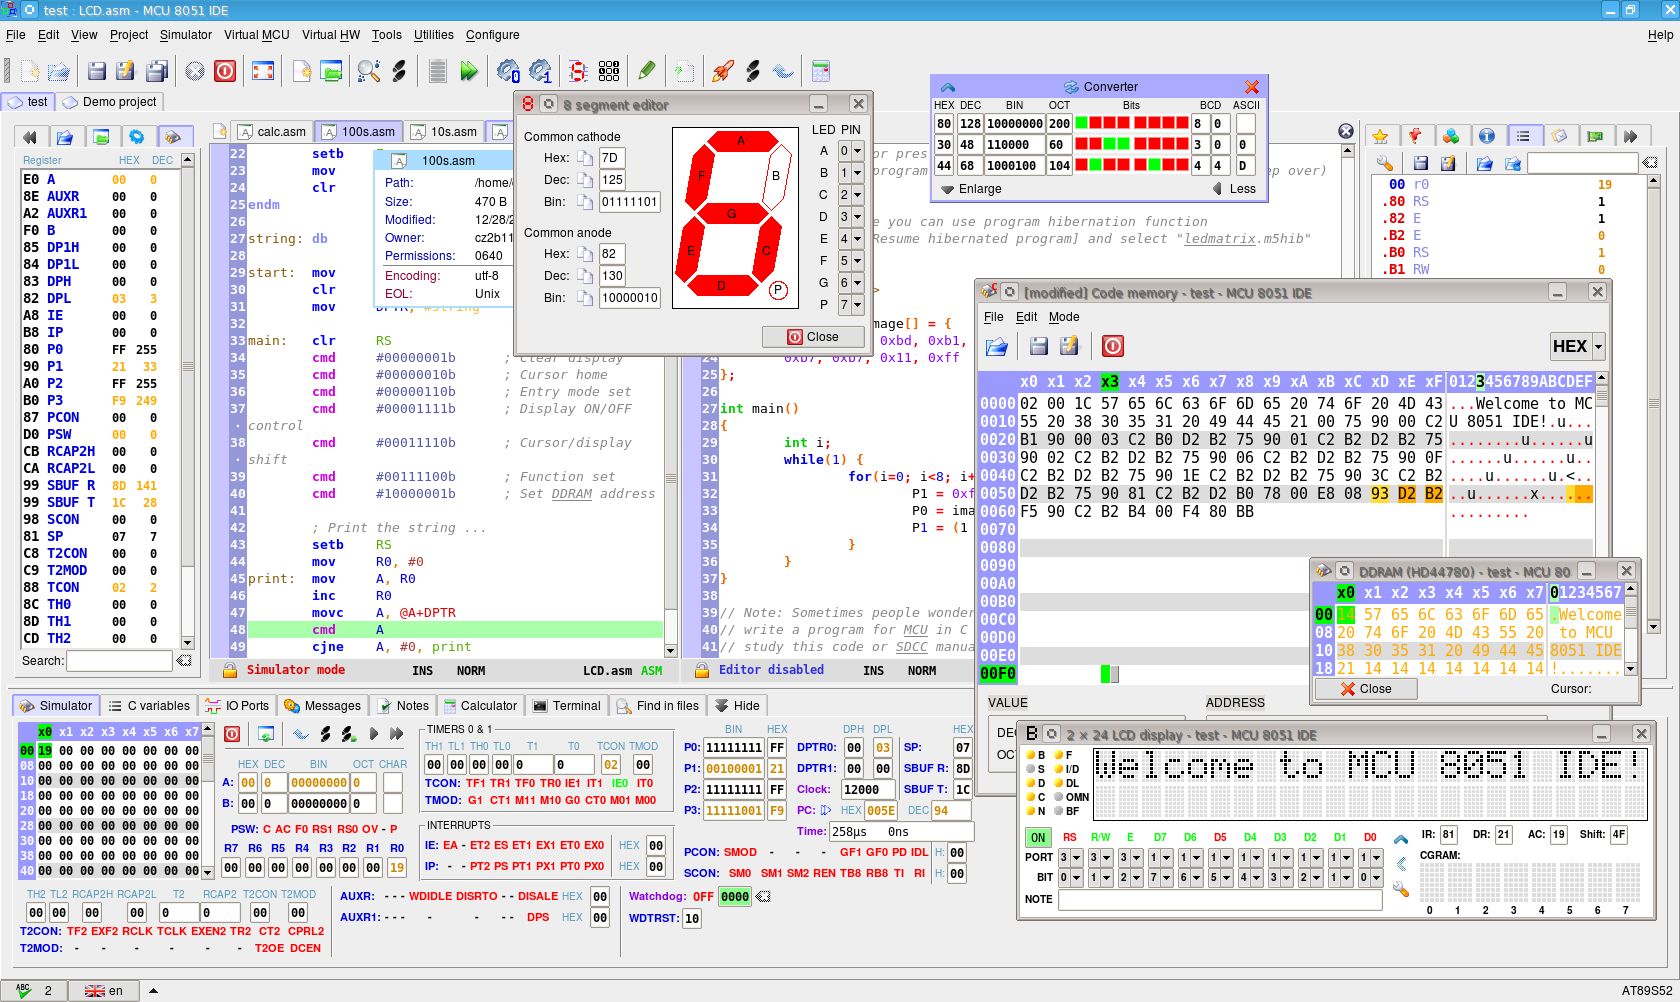
\includegraphics[width=\textwidth]{mcu8051ide.png}
		\captionof{figure}[MCU 8051 IDE]{MCU 8051 IDE} 
	\end{center}
	
	Die Simulation ist eine Softwarekomponente zur Simulation des Mikrocontrollers in einer virtuellen Umgebung. Zusätzliche Features erweitern die Möglichkeit den Mikrocontroller zu simulieren. Beispielsweise gibt es Hardware-Komponenten wie Schalter, Timer und Temperatur Sensor.